% !TEX root = index.tex
\section{Topological Preliminaries}
\setlength{\epigraphwidth}{0.41\textwidth}
\epigraph{Humpty Dumpty sat on a wall,\\
	Humpty Dumpty had a great fall.\\
	All the king's horses and all the king's men\\
	Could not put Humpty together again.}{}

The first step is to break a space up into \emph{simpler spaces} and try to \emph{glue} the pieces back. Simpler spaces will mean contractible spaces and gluing back will be done using locally constant functions.
\begin{align*}
 \xymatrix@R-2pc{
 X \ar@{~>}[r] & \U \\
 \mbox{Topological Space} & \mbox{Good cover of } X
 }
\end{align*}
\begin{definition}
	A topological space\footnote{For us a topological space is simply a subset of $ \R^2 $ or $ \R^3$.} $ X$ is said to be \textbf{contractible} if there exists a point $ x_0 \in X$ and a continuous map
	\begin{align*}
		\Phi: X \times [0,1] \rightarrow X
	\end{align*}
	such that
	\begin{align*}
		\Phi(x,0) & = x   \\
		\Phi(x,1) & = x_0
	\end{align*}
	for all $ x \in X$ i.e. there are ``continuously varying paths'' connecting each point in $ X$ to $ x_0$.
\end{definition}

\begin{figure}[H]
	\centering
	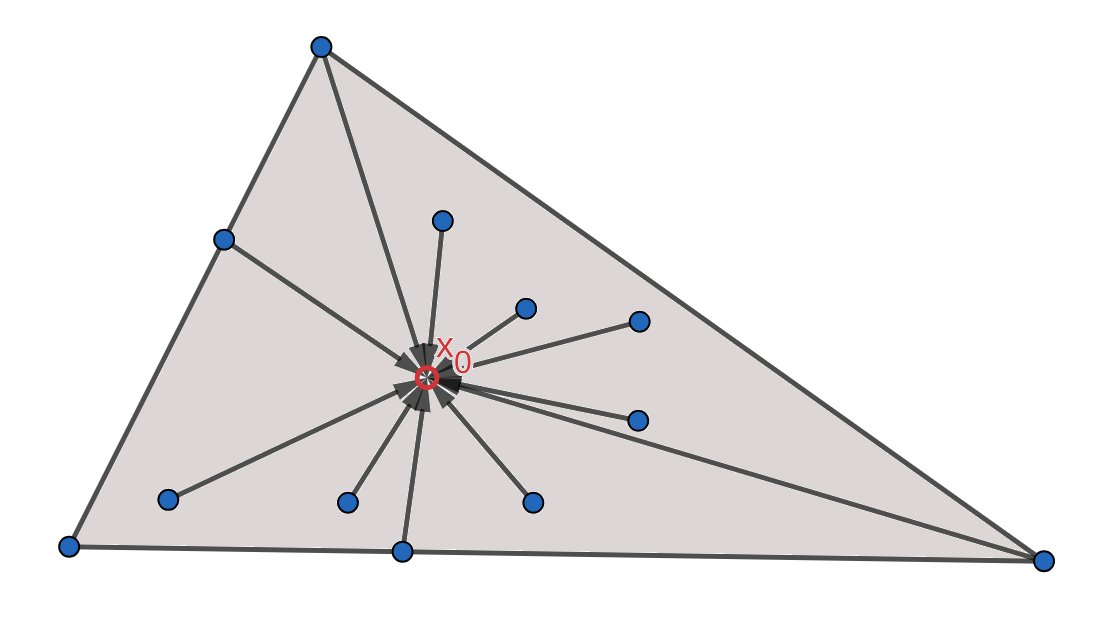
\includegraphics[width=6cm]{contractible}
	\caption{The interior of a triangle is a contractible space.}
\end{figure}

In some sense, a contractible space is as simple a space as is topologically possible. Most algebro-topological invariants cannot distinguish a contractible space from a point. This makes contractible spaces very useful as one may need infinitely many points to \emph{construct} a space but only finitely many contractible spaces to do so, as we'll see below.\\

\begin{ques}
	A subset $ X$ of $ \R^n$ is said to be \textbf{star-shaped} if there exists a point $x_0$ such that for any other point $x \in X$ the segment connecting $x$ to $x_0$ lies entirely in $ X$. Prove that star-shaped subsets of $\R^n$ are contractible.
\end{ques}
\begin{remark}
	This proves that the sets $\R^n$, $ [0,1]$ , $(0,1) $, union of $ x$ and $ y$ axis in $ \R^2$, interior of a convex polygon in $\R^2$, interior of a convex polyhedron in $\R^3$ are all contractible.
\end{remark}
	Not every space is contractible, otherwise topology would have been a very boring subject (which it isn't). The first application of Cech Cohomology will be proving that spaces like the circle $ S^1$, the spheres $ S^2$, $ S^n$, torus, projective space, other higher genus surfaces are {not} contractible.\\

	\begin{ques} Let $X$, $Y$ be topological spaces.
		\begin{enumerate}
			\item Show that if $X$, $Y$ are contractible then so is $X \times Y$. In particular, if $ X$ is contractible then so is $ X \times [0,1]$.
			\item Show that if $ X \times Y$ is contractible, then so is $ X$.
			\item* A subspace $ A \subseteq X$ is said to be a \textbf{retract} of $ X$ if there exists a continuous map $$ r: X \rightarrow A$$ such that $ r(a) = a$ for all $ a \in A$. Show that if $ X$ is contractible and $ A $ is a retract of $ X$ then $ A$ is also contractible.
			\item Is it true that every subset of a contractible space is contractible?
		\end{enumerate}
	\end{ques}

	\begin{definition}
		We say that $X$ is \textbf{connected}\footnote{Technical point: This should really be called \emph{path-connected} but we will only be dealing with spaces where the two notions coincide.} if for any two points $ x_0,x_1 \in X$ there exists a continuous map $ c:[0,1] \rightarrow X$ such that $ c(0) = x_0$ and $ c(1) = x_1$. Define a relation on the set $X$ as $x_0 \sim_{conn} x_1$ if there exists a path in $X$ connecting $x_0$ to $x_1$.
	\end{definition}
	\begin{ques} Let $X$ be a topological space.
		\begin{enumerate}
			\item Show that if $ X$ is contractible then $ X$ is connected.
			\item Show that $\sim_{conn}$ is an equivalence relation.
		\end{enumerate}
	\end{ques}
	\begin{definition}
		Define the \textbf{connected components} of $X$, denoted $\pi_0(X)$, to be the equivalence classes of $X$ under $\sim_{conn}$.
	\end{definition}
	\begin{remark}
		All our spaces will have finitely many connected components.
	\end{remark}

\newpage
\subsection{Covers}
\begin{definition}
	A finite collection of open subsets\footnote{We'll sometimes be lazy and use simplices instead of open subsets.} $ \U = \{ U_1, U_2, \dots, U_n\}$ of a topological space $ X$ is said to be a \textbf{cover} of $ X$ if $X = U_1 \cup U_2 \cup \dots \cup U_n$.
\end{definition}

\begin{example}$ $
	\begin{enumerate}
		\item $ \U = \{ X \}$ is always a cover of $ X$ of any space $X$.
		\item If $ X$ is a triangle, then $ \U = \{ U_1, U_2, U_3\} $ with $ U_i$ being a ``side'' of the triangle is a cover of $ X$.
	\end{enumerate}
\end{example}
\noindent Not all covers are equal. We need the covers to satisfy the following extra condition.
\begin{definition}Let $ [n] = \{ 1, 2, \cdots, n \}$.
	To every non-empty subset $ I \subseteq [n]$ we can associate a subset $U_I$ of $ X$ defined as
	\begin{align*}
		U_I := \bigcap_{i \in I} U_i
	\end{align*}
	The cover $ \U = \{ U_1, U_2, \dots, U_n\}$ is said to be a \textbf{good cover} if for every non-empty subset $ I \subseteq [n]$ every connected component of the space $ U_I$ is contractible.
\end{definition}
\begin{remark}
	In the above definition, $U_I$ can be empty as every connected component of an empty set is contractible.
\end{remark}
\begin{definition}
	The \textbf{dimension} of a cover $ \U $ is the largest $k$ such that there exists some $I \subseteq [n]$ with $|I| = k+1$ and $U_I$ non-empty.
\end{definition}
\begin{figure}[H]
	\centering
	\begin{tikzpicture}[scale=0.6]
		%% vertices
		\draw[fill=black] (0,0) circle (3pt);
		\draw[fill=black] (4,0) circle (3pt);
		\draw[fill=black] (2,3) circle (3pt);
		%% vertex labels
		\node at (2,-0.5) {$U_1$};
		\node at (0.5,1.75) {$U_2$};
		\node at (3.5,1.75) {$U_3$};
		\node at (2,-0.5) {$U_1$};
		\node at (-1,0) {$U_{\{1,2\}}$};
		\node at (5,0) {$U_{\{1,3\}}$};
		\node at (2,3.5) {$U_{\{2,3\}}$};
		%%% edges
		\draw[thick] (0,0) -- (4,0) -- (2,3) -- (0,0);
	\end{tikzpicture}
	\caption{The set of ``sides'' $\U = \{U_1, U_2, U_3\}$ is a good cover of the triangle. In this case $U_{\{1,2\}} = U_1 \cap U_2$, $U_{\{2,3\}} = U_2 \cap U_3$, $U_{\{1,3\}} = U_1 \cap U_3$ are the vertices and $U_{\{1,2,3\}} = U_1 \cap U_2 \cap U_3$ is empty.}
\end{figure}
\newpage
\begin{remark}
	For the following problems, construct good covers with the least possible dimension; the higher the dimension of the cover, the harder the cohomology computations.
\end{remark}
\begin{ques}
	Construct good covers of the following spaces. It's enough (and recommended) to simply draw pictures.
	\begin{multicols}{2}
		\begin{enumerate}
			\item $ \R^n$
			\item $ S^1$ (= the circle)
			\item A Tree
			\item The bipartite graph $ K_{2,3}$
			\item $ \R^2 \setminus \{(0,0) \}$
			\item $ \R^2 \setminus \{(0,0), (1,0), \dots, (k,0) \}$ for some positive integer $ k$
			\item $ S^2$ (= the sphere)
			\item $ S^2 $ minus a point
			\item $ S^2 $ minus 2 points
		\end{enumerate}
	\end{multicols}
\end{ques}

\begin{ques} Find good covers of
	\begin{enumerate}
		\item $S^1 \vee S^1$ = two circles glued at a point (pronounced 'S one wedge S one')
		\item Bouquet of $n$-circles\\
		\begin{tikzpicture}[scale=0.6]
			\begin{polaraxis}[grid=none, axis lines=none]
				\addplot[mark=none,domain=0:360,samples=300] { abs(cos(8*x/2))};
			\end{polaraxis}
		\end{tikzpicture}
		\item $S^1 \vee S^2$ = a circle and a sphere glued at a point (pronounced 'S one wedge S two')
	\end{enumerate}
\end{ques}

\begin{ques}*
	Let $X$, $X'$ be topological spaces with good covers $\U$, $\U'$ respectively. Find a good cover of $X \times X'$. Find a good cover of $S^1 \times S^1$ (= torus). Draw a picture.
\end{ques}

\begin{ques}*
	Find a good cover of the solid torus (which is homeomorphic to $[0,1] \times [0,1] \times S^1$).
\end{ques}

\begin{ques}**
	Find a good cover of the $g$-holed torus.
\end{ques}
It is not true that all spaces admit good covers. However, the spaces that do not admit one are very exotic in nature. For example, every smooth manifold admits a good cover (this is called the Nerve Lemma) however this is false if we drop the adjective smooth. For this class we'll assume that all the spaces under consideration admit a good cover.
